%\documentclass[presentation]{beamer}
\documentclass{beamer}
%\documentclass[notes=hide]{beamer}
%\documentclass[notes=only]{beamer}

\usepackage[title={Lexical affixes in Wao Terero depend on context for properties associated with the lexical-grammatical dichotomy}, creator={Noah Diewald\\Ohio State University\\\texttt{diewald.21@osu.edu}}]{morphologyslides}

%\setbeameroption{show notes on second screen}

\setbeamertemplate{itemize items}{\textcolor{gray}{·}}

\begin{document}

\maketitle

\begin{frame}{What do Wao Terero lexical suffixes contribute to the notion of lexical versus grammatical linguistic content?}

  The lexical-grammatical dichotomy has proven difficult to measure in a consistent manner across languages, or even within any single language.

  \vfill
  
  There is also major disagreement among linguists concerning what should be considered lexical or grammatical.

\end{frame}
  
\begin{frame}{Are there diagnostics that unambiguously measure the grammatical-lexical contrast?}
  
  I explore a measure of grammaticality that relies on relative discourse status.

  \vfill

  \citet{Boye2012, Boye2023} propose that categorically grammatical items have conventionally secondary discourse status, while lexical items are capable of having primary status.

\end{frame}

\begin{frame}{I extend the diagnostics of Boye and Harder for measurements of fine-grained morphological meanings.}
  
  I utilize the negation diagnostic borrowed from the literature on \emph{proffered content} to measure the discourse primary status of meanings.

  \vfill

  Proffered content is what is asserted in an assertion, and is the non-presupposed content of questions and commands \citep{Roberts2012}.

\end{frame}

\begin{frame}{I demonstrate that based on that measure, the discourse status of Wao Terero lexical suffixes is not item specific but context specific.}
  
  In realizational terms, the same morph may be licensed in either a lexical or grammatical context.

\end{frame}

\begin{frame}{This means that morphemes are not categorically either lexical or grammatical.}

  There are theories that emphasize a dichotomy, such as Distributed Morphology \citep{Bobaljik2017}, where some morphological forms are grammatically licensed, while others are strictly associated with lexical \dmroot{}s.

  \vfill
  
  This does not predict the distribution of Wao Terero lexical suffixes in all their uses.
  
\end{frame}

\begin{frame}{Data is drawn from my fieldwork with Wao Terero speakers.}

  Wao Terero is a linguistic isolate spoken in the Ecuadorian Amazon.

  \centering
  
\includegraphics[width=3in]{consultants.jpg}

  \footnotesize Some fieldwork consultants in my office in Puyo, Ecuador.
\end{frame}

\begin{frame}{I begin with an overview of data.}

  My goals are the following:
  
  \begin{itemize}
  \item The examples allow for an understanding of the data used in later diagnostics.
  \item Lexical suffixes and their uses are shown to be correctly classified in my description.
  \item Additional argumentation relevant to grammatical status provides convergent data points that lend strength to the validity of the discourse-based diagnostics.
  \end{itemize}

\end{frame}

\begin{frame}{I use a number of non-standard glossing conventions.}

  These are largely to focus attention on aspects of examples that are key to arguments made in this work.

  \begin{itemize}
  \item \lxr{plant}: Bound stems with little or no independent meaning have labeled glosses placed in parentheses. The label does not represent a meaning. They are de-emphasized in size and color.
  \item \lx{ls}\lxa{plant}: For lexical suffixes generally. They are annotated with a label, which is de-emphasized and does not, necessarily, correspond to a semantic interpretation.
  \item \lx{clf}\lxa{plant}: For classifier uses of lexical suffixes.
  \end{itemize}
  
\end{frame}

\begin{frame}{Lexical suffixes have a wide distribution.}

  The suffixes occur on most parts of speech, including:

  \begin{itemize}
  \item nouns,
  \item verbs,
  \item adjectives,
  \item demonstratives,
  \item numerals,
  \item quantifiers,
  \item and question words.
  \end{itemize}

  \vfill
  
  I leverage this diversity to make a comparison of their lexical versus grammatical uses across categories.
  
\end{frame}

\begin{frame}{Lexical suffixes in Wao Terero are a closed class.}

  Documentation is ongoing. The longest list of affixes includes 80 \citep{Fiddler2011}\footnote{The list is taken from an unpublished manuscript by Catherine Peeke.}.
  I find at least 33 of these to be questionable for various reasons.
  Whatever the precise size of the class, there is no productive means of adding to it.

\end{frame}

\begin{frame}{On nominals, lexical suffixes are associated with nominal meanings that are sometimes compound-like.}
  
  \pex
  \a\begingl
  \gla kẽ-wẽ //
  \glb \lxr{manioc}-\lx{ls}\lxa{plant} //
  \glft \gl{manioc plant/stalk/stem} //
  \endgl
  \a\begingl
  \gla kẽ-dẽ //
  \glb \lxr{manioc}-\lx{ls}\lxa{food} //
  \glft \gl{manioc tuber} //
  \endgl
  \a\begingl
  \gla kẽ-wẽ-yabo //
  \glb \lxr{manioc}-\lx{ls}\lxa{plant}-\lx{ls}\lxa{leaf} //
  \glft \gl{manioc leaf} //
  \endgl
  \xe

  Described by \citet{Peeke1968} as \emph{classifiers}, nominal uses demonstrate a distribution consistent with lexical suffixes in other languages \citep{Haeberlin1974}.

\end{frame}

\begin{frame}{For nominals, lexical suffixes are not in competition.}

  \ex
  \begingl
  \gla kẽ-wẽ-yabo //
  \glb \lxr{manioc}-\lx{ls}\lxa{plant}-\lx{ls}\lxa{leaf} //
  \glft \gl{manioc leaf} //
  \endgl
  \xe

  This might imply they are more like common nouns in compounds, which do not compete and are considered lexical.
\end{frame}

\begin{frame}{Some nominal stems are bound and contribute little to meanings.}

  These will prove key in demonstrating certain aspects of the lexical-grammatical status of the suffixes.

  \vfill
  
  There are two types of interest.
  
\end{frame}

\begin{frame}{First, there are stems that occurs with only a particular affix, limiting the affix meaning.}

  \ex
  \begingl
  \gla di-ka //
  \glb \lxr{stone}-\lx{ls}\lxa{fruit} //
  \glft \gl{stone} //
  \endgl
  \xe

  The \wf{-ka} affix is associated with multiple meanings.
  With \wf{di-} it may only be interpreted as \gl{stone}.
  
\end{frame}

\begin{frame}{Second, there are stems that occur with a number of affixes, limiting the affix meaning.}

  \pex
  \a\begingl
  \gla õdõ-boka //
  \glb \lxr{body}-\lx{ls}\lxa{ear} //
  \glft \gl{ear} //
  \endgl
  \a\begingl
  \gla õdõ-po //
  \glb \lxr{body}-\lx{ls}\lxa{hand} //
  \glft \gl{hand} //
  \endgl
  \a\begingl
  \gla õdõ-yabe //
  \glb \lxr{body}-\lx{ls}\lxa{back} //
  \glft \gl{back (of body)} //
  \endgl
  \xe

  The \wf{-po} suffix, in particular, has a range of uses, including \gl{hand}, \gl{forelimb}, \gl{canoe}, and \gl{grape-like cluster}.
\end{frame}

\begin{frame}{On other parts of speech lexical suffixes often have a classifier function.}
  
  \pex
  \a\begingl
  \gla a-wẽ pa-wẽ-ta-bo-pa //
  \glb \lxr{plant}-\lx{ls}\lxa{plant} cut-\lx{clf}\lxa{plant}-\lx{pst}-\lx{1}-\lx{decl} //
  \glft \gl{I was cutting trees.} //
  \endgl
  \a\begingl
  \gla bãdĩ-ka di-ka a-bo-pa //
  \glb \lx{dem}-\lx{clf}\lxa{fruit} \lxr{stone}-\lx{ls}\lxa{fruit} see-\lx{1}-\lx{decl} //
  \glft \gl{I see this stone.} //
  \endgl
  \xe

  As evidence of classifier status, one sees characteristic ``doubling'', where the affix constrains felicitous arguments of the host but does not \emph{saturate} the argument \citep{Mithun1986, Rosen1998}.
  
\end{frame}

\begin{frame}{The classifier function is unlike grammatical agreement.}

  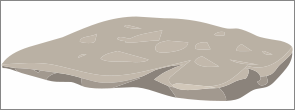
\includegraphics[width=1in]{flatstone.png}

  \pex
  \a\begingl
  \gla bãdĩ-pa di-ka a-bo-pa //
  \glb \lx{dem}-\lx{clf}\lxa{board} \lxr{stone}-\lx{ls}\lxa{fruit} see-\lx{1}-\lx{decl} //
  \glft \gl{I see this stone. (when the stone is flat)} //
  \endgl
  \a\begingl
  \gla bãdĩ di-ka a-bo-pa //
  \glb \lx{dem} \lxr{stone}-\lx{ls}\lxa{fruit} see-\lx{1}-\lx{decl} //
  \glft \gl{I see this stone.} //
  \endgl
  \xe

  Unlike grammatical agreement, classifier use shows \emph{semantic} concord, and is not obligatory.
  
\end{frame}

% \begin{frame}{Classifiers may be taking on more agreement-like qualities.}
%    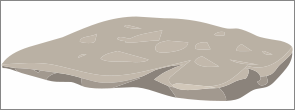
\includegraphics[width=1in]{flatstone.png}

%   \pex
%   \a\label{one}\begingl
%   \gla bãdĩ-pa di-ka a-bo-pa //
%   \glb \lx{dem}-\lx{clf}\lxa{board} \lxr{stone}-\lx{ls}\lxa{fruit} see-\lx{1}-\lx{decl} //
%   \glft \gl{I see this stone. (when the stone is flat)} //
%   \endgl
%   \a\label{two}\begingl
%   \gla bãdĩ-pa a-bo-pa //
%   \glb \lx{dem}-\lx{clf}\lxa{board} see-\lx{1}-\lx{decl} //
%   \glft \gl{I see this. (when something is flat)} //
%   \endgl
%   \xe

%   One young speaker out of 4, the rest 10-20 years older, disliked (\ref{one}) but accepted (\ref{two}), provided the same picture of a stone for context.
%   The other speakers were her uncles and father, all in separate sessions.
  
% \end{frame}

\begin{frame}{Classifiers exhibit abstract meanings not found in nominal settings.}
  
  \begin{tabular}{ll}
    -ka & head-related, fruit, stone, \emph{round} \\
    -pa & wooden, board, projectile, \emph{flat} \\
    -we & pole, plant, branch, tree, \emph{long and cylindrical} \\
  \end{tabular}

  \pex
  \a\judge{\#/*}\begingl
  \gla kẽ-dẽ-ka //
  \glb \lxr{manioc}-\lx{ls}\lxa{food}-\lx{ls}\lxa{fruit} //
  \glft \gl{round manioc tuber} //
  \endgl
  \a\begingl
  \gla bãdĩ-ka kẽ-dẽ //
  \glb \lx{dem}-\lx{clf}\lxa{fruit} \lxr{manioc}-\lx{ls}\lxa{food} //
  \glft \gl{this (round) manioc tuber} //
  \endgl
  \xe

\end{frame}

% \begin{frame}{Not all lexical suffix usage with non-nominals is classifier-like.}
  
%   \pex
%   \a\begingl
%   \gla yẽdẽ-gade yede-kã ba-kã-pa //
%   \glb big-\lx{ls}.stomach big-3.\lx{h} remain-3.\lx{h}-\lx{decl} //
%   \glft \gl{The fat person will remain fat.}//
%   \endgl
%   \a\begingl
%   \gla godõ-bõka-te //
%   \glb pull-\lx{ls}.ear-\lx{ger} //
%   \glft \gl{listening} \trailingcitation{\citep[pp.~161]{Pike1988}} //
%   \endgl
%   \xe

% \end{frame}

% \begin{frame}{On verbs, adjectives, and demonstratives, lexical suffixes are always in competition (verb example).}

%   \pex
%   \a\begingl
%   \gla õdõ-po-gõ kẽ-po-bo-pa yebẽ-ka //
%   \glb \lxr{body}-\lx{ls}\lxa{hand}-\lx{ls}\lxa{thorn} cut-\lx{clf}\lxa{hand}-1-\lx{decl} machete-\lx{inst} //
%   \glft \gl{I cut my finger with a machete.} //
%   \endgl
%   \a\ljudge{*}\begingl
%   \gla õdõ-po-gõ kẽ-po-gõ-bo-pa yebẽ-ka //
%   \glb \lxr{body}-\lx{ls}\lxa{hand}-\lx{ls}\lxa{thorn} cut-\lx{clf}\lxa{hand}-\lx{clf}\lxa{thorn}-1-\lx{decl} machete-\lx{inst} //
%   \glft \gl{I cut my finger with a machete.} //
%   \endgl
%   \xe

%   Competition, even when the semantics might motivate the occurrence of multiple items, is a grammatical characteristic.

% \end{frame}
  
\begin{frame}{On verbs, adjectives, and demonstratives, lexical suffixes are always in competition.}

  \pex
  \a\begingl
  \gla yẽdẽ-po õdõ-po-gõ a-bo-pa //
  \glb big-\lx{clf}\lxa{hand} \lxr{body}-\lx{ls}\lxa{hand}-\lx{ls}\lxa{thorn} see-1-\lx{decl} //
  \glft \gl{I see a big finger.} //
  \endgl
  \a\ljudge{*}\begingl
  \gla yẽdẽ-po-gõ õdõ-po-gõ a-bo-pa //
  \glb big-\lx{clf}\lxa{hand}-\lx{clf}\lxa{thorn} \lxr{body}-\lx{ls}\lxa{hand}-\lx{ls}\lxa{thorn} see-1-\lx{decl} //
  \glft \gl{I see a big finger.} //
  \endgl
  \xe

  Competition, even when the semantics might motivate the occurrence of multiple items, is a grammatical characteristic.

\end{frame}

% \begin{frame}{On verbs, lexical suffixes are not in competition with person marking.}

%   \ex\judge{*/\#}\begingl
%   \gla ĩ-kã ĩ-kã-te kẽ-kã-bo-pa yebẽ-ka //
%   \glb \lx{pro}-3.\lx{h} \lx{cop}-3.\lx{h}-\lx{acc} cut-3.\lx{h}-1-\lx{decl} machete-\lx{inst} //
%   \glft \gl{I cut him with a machete.} //
%   \endgl
%   \xe

%   The classifier position is specific to concord with non-sentient arguments that are non-subjects.
%   The person position is specific to concord with sentient subjects.

%   \vfill
  
%   An alternative view may be that the lexical and non-lexical cannot compete.
%   One may leverage the distributional diversity of the system to determine if this is the case.
  
% \end{frame}

% \begin{frame}{"Dual use" affixes, with both a person interpretation and another interpretation, may occur in lexical suffix position with a non-person interpretation.}

%   \ex\begingl
%   \gla baõ-kã kẽ-kã-bo-pa yebẽ-ka //
%   \glb \lxr{body}-\lx{ls}\lxa{body} cut-\lx{clf}\lxa{body}-1-\lx{decl} machete-\lx{inst} //
%   \glft \gl{I cut my body with a machete.} //
%   \endgl
%   \xe

%   Notably, there is no person marking for non-sentient animals and inanimates in Wao Terero.
%   This provides an alternative to lexical versus grammatical in describing the role the positions may be sensitive to.

% \end{frame}

\begin{frame}{In adjectives, demonstratives and other parts of speech, person marking and lexical suffixes are in competition.}

  \pex
  \a\begingl
  \gla yẽdẽ-gade ĩ-dã-pa //
  \glb big-\lx{clf}\lxa{stomach} \lx{cop}-3.\lx{f}-\lx{decl} //
  \glft \gl{She is fat.}//
  \endgl
  \a\begingl
  \gla yẽdẽ-dã ĩ-dã-pa //
  \glb big-3.\lx{f} \lx{cop}-3.\lx{f}-\lx{decl} //
  \glft \gl{She is fat.}//
  \endgl
  \a\ljudge{*}\begingl
  \gla yẽdẽ-gade-dã ĩ-dã-pa //
  \glb big-\lx{clf}\lxa{stomach}-3.\lx{f} \lx{cop}-3.\lx{f}-\lx{decl} //
  \glft \gl{She is fat.}//
  \endgl
  \xe
  
\end{frame}

\begin{frame}{How do we measure the grammatical versus lexical status of the suffixes?}

  The following discussion of diagnostics has three goals.
  
  \begin{itemize}
  \item The definitions and diagnostics provided by \citet{Boye2012} are presented.
  \item Issues with the original diagnostics are discussed.
  \item The negation diagnostic for proffered content is described.
  \end{itemize}
\end{frame}

\begin{frame}{The Boye and Harder provide the following definitions of lexical and grammatical meaning.}
  \begin{itemize}
  \item {\scshape Lexical meaning}: Lexical meaning is by convention capable of being discursively primary.
  \item {\scshape Grammatical meaning}: Grammatical meaning is by convention discursively secondary.
  \end{itemize}
\end{frame}

\begin{frame}{There are two proposed symptoms of secondary status.}

  \begin{itemize}
  \item {\scshape Nonfocalizability as symptom of grammatical status}: Grammatical expressions cannot be assigned discursively primary status by focalizing expressions. \citep[p.~14]{Boye2012}
  \item {\scshape Nonaddressability as symptom of grammatical status}: Grammatical expressions cannot be assigned discursively primary status by being addressed in subsequent discourse. \citep[p.~15]{Boye2012}
  \end{itemize}
\end{frame}

\begin{frame}{The issue with the tests for these symptoms is that they also serve as word-hood and constituency tests.}

  Nonaddressability is one half of the notion of an \emph{anaphoric island}, and exists in various definitions of lexical integrity \citep{Simpson1991}.

  \vfill
  
  ``[S]uch an entity is a sentence part which cannot contain an anaphoric element whose antecedent lies outside the part in question and \emph{which cannot contain the antecedent structure for anaphoric elements lying outside}.'' \citep[p.~205]{Postal1969}

  \vfill
  
  The domain of the word is argued to have this characteristic.\footnote{
  See \citet{Harris2006} for arguments for non-English counter examples.}
  
\end{frame}

\begin{frame}{Nonfocalizability diagnostics are also biased toward whole word forms.}

  The proposed diagnostics focus on English, such as cleft constructions, and occurrence within the scope of particles such as \wf{only}, \wf{just}, or \wf{even}.
  These are only appropriate for items that are not bound.

  \vfill

  There is a narrow focus test but using this to focus sub-word components is considered meta-linguistic.
\end{frame}

\begin{frame}{As a measure of discourse primary status, negation diagnostics behave similarly to the Boye and Harder diagnostics for many items.}

  \ex It is not the case that Fluffy, a cat, saw birds. \xe
  
  A common noun may be discourse secondary in some contexts, where it is not canceled under negation.
  
  \ex It is not the case that a cat saw dogs. \xe

  But a common noun is \emph{capable} of being primary, and may be canceled.
  This indicates that its meaning is lexical.

  \vfill
  
  Tense, number, gender, etc.\ cannot be canceled in this way.
  This indicates that they are conventionally secondary, and therefore grammatical.
\end{frame}

% \begin{frame}{\citet{Boye2023} aligns the notion of \emph{at-issue} with discourse primary status.}

%   The notion of \emph{at issue} is related to \emph{proffered content} \citep{Roberts2012}.
%   Both correspond to foregrounded content.
%   The major difference is that \emph{at-issue} content may include non-conventional content, such as conversational implicatures \citep{Roberts2009}.
  
% \end{frame}

% \begin{frame}{Proffered content is foreground content.}

%   It is what is asserted in an assertion, and is the non-presupposed content of questions and commands \citep{Roberts2012}.
  
% \end{frame}

% \begin{frame}{Diagnostics for proffered content are well established.}
%   By linking the notion of discourse primary with proffered, there are a large host of existing diagnostics that can be employed, which do not rely on criteria closely associated with non-bound status.

%   \vfill

%   I will use the negation diagnostic.
% \end{frame}

% \begin{frame}{Negation cancels proffered content under its scope.}

%   \pex
%   \a A: The boys walked home, yesterday.
%   \a B: No, they ran.
%   \a B: No, it was Sally.
%   \a B: No, it was Friday.
%   \xe

%   There are certain meanings that may be directly negated.
%   These include the identity of the walker(s), the action performed, and the precise time offered.  
% \end{frame}

% \begin{frame}{Negation does not cancel non-proffered content.}
%   \pex
%   \a A: The boys walked home, yesterday.
%   \a B: No, they are not the boys. 
%   \xe

%   The notion that there are specific, familiar \wf{boys}, is not canceled by direct negation.
%   Likewise, there is no way to specifically, target the plurality of the boys, or the verb tense.
% \end{frame}

% \begin{frame}{Some content is non-proffered only in some contexts.}
%   \pex
%   \a A: I see boys.
%   \a B: No, they are not boys.
%   \a\judge{\#} B: No, it is not boys.
%   \xe
  
%   This indicates that \wf{boys} are capable of being discourse primary, and the meaning is lexical.

%   \vfill

%   There is no way to cancel plurality by direct negation, meaning it is grammatical.
% \end{frame}

\begin{frame}{The negation diagnostic differs in its ability to target fine grained meanings.}

  \citet{Boye2012} consider pronouns to be lexical due to focalizability.
  
  \pex
  \a A: Is that him?
  \a B: No, it isn't him. He is at home.
  \xe

  Placing \wf{him} within the scope of negation does not cancel gender, number, the familiarity of the referent, nor the target of the referent.
  Therefore, these meanings of the pronoun, are non-proffered.

\end{frame}

\begin{frame}{This does not contract Boye and Harder's claim.}

  The diagnostic adds nuance.
  A pronoun is a mixture of lexical and grammatical meanings.
  
  \vfill

  ``The proffered content of a pronoun is just a variable whose semantic value in a particular context is always given in the same way, via a contextually specified function assigning values to variables.'' \citep[p.~504]{Roberts2004}
\end{frame}

\begin{frame}{It is now time to test Wao Terero constructions.}
  There are three parts to this.

  \begin{itemize}
  \item The grammatical status of classifiers will be demonstrated.
  \item It will be established that sometimes lexical suffix meanings may be proffered.
  \item An argument is made as to why this is different than common nouns in English.
  \end{itemize}
\end{frame}

\begin{frame}{To test whether classifiers are proffered content, I utilize a "true, false, nonsense" paradigm.}
  \pex\label{rock1} {\bf context:} Given the image, are the following statements true, false or nonsense?\newline
  \includegraphics[width=0.5in]{/home/noah/Documents/writing/figures/small-stone-above.png}
  \a\ljudge{T}\begingl
  \gla gītã-ka eibe ĩ-pa //
  \glb small-\lx{clf}\lxa{fruit} above \lx{cop}-\lx{decl} //
  \glft \gl{The small one is above.} //
  \endgl
  \a\ljudge{F}\begingl
  \gla yẽdẽ-ka eibe ĩ-pa //
  \glb big-\lx{clf}\lxa{fruit} above \lx{cop}-\lx{decl} //
  \glft \gl{The big one is above.} //
  \endgl
  \xe
 
\end{frame}

\begin{frame}{Improper classifier use results in infelicity.}

  \pex {\bf context:} Given the image, are the following statements true, false or nonsense?\newline
  \includegraphics[width=0.5in]{/home/noah/Documents/writing/figures/small-stone-above.png}
  \a\ljudge{\#}\begingl
  \gla gītã-wẽ eibe ĩ-pa //
  \glb small-\lx{clf}\lxa{plant} above \lx{cop}-\lx{decl} //
  \glft \gl{The small one is above.} //
  \endgl
  \a\ljudge{\#}\begingl
  \gla yẽdẽ-wẽ eibe ĩ-pa //
  \glb big-\lx{clf}\lxa{plant} above \lx{cop}-\lx{decl} //
  \glft \gl{The big one is above.} //
  \endgl
  \xe
\end{frame}

\begin{frame}{Negation does not cancel classifier meanings.}
  
  \pex\label{rock1} \includegraphics[width=0.5in]{/home/noah/Documents/writing/figures/small-stone-above.png}
  \a\ljudge{F}\begingl
  \gla gītã-ka eibe ĩ-dãbai ĩ-pa //
  \glb small-\lx{clf}\lxa{fruit} above \lx{cop}-\lx{neg} \lx{cop}-\lx{decl} //
  \glft \gl{The small one is not above.} //
  \endgl
  \a\ljudge{T}\begingl
  \gla yẽdẽ-ka eibe ĩ-dãbai ĩ-pa //
  \glb big-\lx{clf}\lxa{fruit} above \lx{cop}-\lx{neg} \lx{cop}-\lx{decl} //
  \glft \gl{The big one is not above.} //
  \endgl
  \xe

  Reference is felicitous and is not canceled despite being under the scope of negation.
\end{frame}

\begin{frame}{Classifiers meanings appear to be grammatical.}

  I have yet to discover any means of directly negating a classifier.
  
\end{frame}

\begin{frame}{Are nominal uses also grammatical?}

  Compound-like constructions are difficult.
  \wf{Strawberry} is not really related to \gl{straw}, and is only a type of \wf{berry}.
  Demonstrating that these can be negated independently is not informative for the idiomatic compound.
  
\end{frame}

\begin{frame}{Negation can be tested with "meaningless" stems.}
  I do not perform in depth diagnostics on these because the result is fairly obvious.
 
  \pex
  \a\begingl
  \gla di-ka a-dãbai ĩ-bo-pa //
  \glb \lxr{stone}-\lx{ls}\lxa{fruit} see-\lx{neg} \lx{cop}-1-\lx{decl} //
  \glft \gl{I don't see a stone.} //
  \endgl
  \xe
  
  A meaning of \wf{-ka} is \gl{stone}.
  The stem \wf{di-} does not add anything but a restriction on possible meanings in \wf{di-ka}.
  One of the meanings of \wf{-ka} was primary in this construction.
\end{frame}

\begin{frame}{Body-parts meanings can generally become primary with \wf{õdõ}.}
 
  \pex
  \a\begingl
  \gla õdõ-po a-dãbai ĩ-bo-pa //
  \glb \lxr{body}-\lx{ls}\lxa{hand} see-\lx{neg} \lx{cop}-1-\lx{decl} //
  \glft \gl{I don't see a hand.} //
  \endgl
  \xe
  
\end{frame}

% \begin{frame}{Not all body part meanings can be made primary.}

%   \begin{tabular}{lll}
%     * õdõ-ka & & head \\
%     * o-ka & & head \\
%     o-ka-bõ & \lxr{head}-\lx{ls}\lxa{fruit}-\lx{ls}\lxa{seed} & head \\
%     o-ka-ta & \lxr{head}-\lx{ls}\lxa{fruit}-\lx{ls}\lxa{claw} & skull \\
%     o-ka-gi & \lxr{head}-\lx{ls}\lxa{fruit}-\lx{ls}\lxa{string} & hair \\
%     awĩ-ka & \lxr{eye}-\lx{ls}\lxa{fruit} & eye/face \\
%   \end{tabular}

%   \vfill
  
%   The \wf{-ka} affix cannot mean \gl{head} in nominals without some additional modification.
%   In nominal uses, as in classifier uses, it is abstractly, \emph{head related}.
% \end{frame}

\begin{frame}{Does this mean that classifiers are lexical, despite their grammatical behavior?}
  According to \citet{Boye2012}, lexical meanings are \emph{capable} of being discourse primary.

  \vfill

  There is no uniform grammatical convention for changing discourse status that applies to the class as a whole.

  \begin{itemize}
  \item There are only some meaningless stems, like \wf{di-}. Not all suffixes have such a stem available to ``promote them''.
  \item Only some meanings are represented in these contexts, such as body-part meanings with \wf{õdõ-}.
  \item Some meanings appear to be only available with classifier uses, such as the \gl{round} meaning of \wf{-ka}.
  \end{itemize}
\end{frame}

\begin{frame}{This is different than nouns in English.}
  
  \pex
  \a The cats/communications/charges accomplished the goal.
  \a I saw cats/communications/charges.
  \xe

  Uniformly across the category of common nouns, the same patterns in relative discourse status occurs in the same grammatical environments, without any restriction on an item's nominal polysemy.

\end{frame}

\begin{frame}{Labeling the affixes as inherently grammatical or lexical has issues.}

  There are two points to support this.
  
  \begin{itemize}
  \item A mixed labeling within the class is redundant.
  \item Labeling the items within the class, uniformly, results in meaning gaps between context types.
  \end{itemize}
\end{frame}

\begin{frame}{It would be extremely redundant for some suffix meanings to have a homophonous lexical duplicate.}
  
  Proposing a lexical \gl{rock} \wf{-ka} when there is a classifier \wf{-ka}, which also has a \gl{rock}-related meaning is redundant.
  Each such lexical morpheme would share a meaning and a form with a grammatical duplicate.

\end{frame}

\begin{frame}{Proposing that all suffixes are lexical and may be converted or embedded in classifier structures does not account for all classifier meanings.}

  Not all lexical suffix meanings occur with nominals.
  Fewer of these are demonstrably capable of being discourse primary.

  \vfill

  \begin{center}
    \begin{tabular}{lll}
      Lexical Meanings & & Converted to Grammatical \\
      \rooted{ka} \gl{stone} & $\to$ & $[_\text{\lx{clf}} \text{\rooted{ka}} ]$ \gl{stone} \\
      \rooted{ka} \gl{fruit} & $\to$ & $[_\text{\lx{clf}} \text{\rooted{ka}} ]$ \gl{fruit} \\
      \rooted{ka} X & ? & $[_\text{\lx{clf}} \text{\rooted{ka}} ]$ \gl{round} \\
    \end{tabular}
  \end{center}

  \vfill

  Where does the \gl{round} meaning come from?

  \vfill
  
  Proposing the opposite conversion direction would predict that the meaning \wf{round} occurs in lexical uses. 
  
\end{frame}

% \begin{frame}{Converting grammatical to lexical does not account for idiomatic compounds.}

%   \pex
%   \a\begingl
%   \gla o-ka-ta //
%   \glb \lxr{head}-\lx{ls}\lxa{fruit}-\lx{ls}\lxa{claw} //
%   \glft \gl{skull} //
%   \endgl
%   \a\begingl
%   \gla bẽkayõ-ta //
%   \glb \lxr{notebook}-\lx{ls}\lxa{claw} //
%   \glft \gl{student/notebook} //
%   \endgl
%   \xe

%   There is some notion of motivation since \wf{-ta} can be associated with shells and paper-like substances.
%   Yet, the ultimate meaning does not suggest a composition of grammatical meanings.
% \end{frame}

\begin{frame}{Categorizing affixes as inherently grammatical or lexical does not predict the behavior of Wao Terero lexical suffixes.}

  This is not to say that a theory like DM, which requires such a categorization, does not allow for analyses of Wao Terero data.
  Popular theories tend to be very flexible and capable of handling diverse phenomena.
  
  \vfill
  
  The point is that such an analysis would not fall out of a theory's morpheme categorization strategy.
  A potential analysis might be possible \emph{despite} the strategy.
  
\end{frame}

\begin{frame}{I propose an alternative explanation to the Wao Terero data.}

  A simple explanation for such a mixed distribution is that lexical and grammatical meanings are in the licensing context, and are not rigid properties of the affixes themselves.
  This may help explain phenomena in other languages where the behavior of some items is ambiguous.

\end{frame}

\begin{frame}{The proposal is consistent with realizational principles.}
  
  The realizational claim is that morphs, the phonological content of a morpheme, are not rigidly paired with meanings.
  Instead, they are licensed according to information that is available in a grammatical-semantic context.

\end{frame}

\begin{frame}{The notion that morphs are blind to the lexical-grammatical dichotomy is a conservative extension of existing ideas.}
  
  The extension of realization analyses to lexical meanings has already been argued for elsewhere \citep{Harley2014}.
  It is only one step further to propose that some morphs may then be licensed in either a lexical or grammatical context.
  
\end{frame}

\begin{frame}{How would such a system work formally?}
  
  This is a topic of my dissertation.
  Unfortunately, it involves a lot of details that I couldn't fit into a 20 minute talk.
  
\end{frame}

\begin{frame}{A final note on lexical and grammatical as categories.}

  Measuring discourse primary versus discourse secondary status can be performed in an unambiguous fashion.

  It may be the case that some are unconvinced of the validity of the measure in relation to grammaticality.
\end{frame}

\begin{frame}{Without a rigid measure we are back to square one.}
  If there is no consensus, perhaps it is not possible to clearly differentiate the categories.

  \vfill

  In that case it makes still less sense to label morphemes as inherently either lexical or grammatical.
\end{frame}

\begin{frame}{Thank you!}

  Thank you also to the consultants, Edo, Toriboi and the Boyotai family, Flora, Nee, Alberto, Rubén, Abraham, Jennifer and Maria.
  Thanks for taking my phone calls when I get confused.

  \vfill

  Initial fieldwork was hosted at the Andes and Amazonian Field School (www.iyarina.org).
  
  \vfill

  \footnotesize
  Portions of this research were funded by the following: Jacobs Research Funds Individual Grant; Lewis and Clark Fund for Exploration and Field Research, American Philosophical Society; Foreign Language and Area Studies Fellowship, Ohio State; International Research and Scholarship Grant, Office of International Affairs, Ohio State University.
  
\end{frame}

\begin{frame}[allowframebreaks]{References}
  \printbibliography
\end{frame}

\end{document}
%%% Local Variables:
%%% mode: latex
%%% TeX-master: t
%%% End:
